% siminos/CLE/Hilbert.tex
% $Author: siminos $ $Date: 2009-12-19 02:59:14 +0100 (Sat, 19 Dec 2009) $

%\subsection{\label{s:Hilbert}Hilbert basis approach}

The most common approach to symmetry reduction is through the
use of a Hilbert basis of invariant polynomials. One computes
a (non-unique) basis of linearly independent polynomials,
invariant under the action of the symmetry group (\cf
\refref{gatermannHab,ChossLaut00} for a discussion of
methods) and either rewrites the dynamics in this basis or
maps the solutions to the polynomials.
The reader is referred to the book of Gilmore and
Lettelier\rf{GL-Gil07b} for a very detailed discussion of
symmetry reduction, through the use of invariant polynomials\ES{Also Chossat and Lauterbach?}.

It will be convenient to rewrite the system in real variables
$x=x_1+ i\, x_2\,,\ y=y_1+i\, x_2$ as
\beq
\begin{split}
	\dot{x}_1 &= -\sigma x_1 + \sigma y_1\cont
	\dot{x}_2 &= -\sigma x_2 + \sigma y_2\cont
	\dot{y}_1 &= (\RerCLor-z) x_1 - \ImrCLor x_2 -y_1-e y_2 \cont
	\dot{y}_2 &= \ImrCLor x_1 + (\RerCLor-z) x_2 + e y_1- y_2\cont
	\dot{z} \; &= -b z + x_1 y_1 + x_2 y_2\,.
	\label{eq:CLeR}
\end{split}
\eeq

The action \refeq{eq:SO2cle} of $\SOn{2}$ on $\Rls{5}$ is then given by
\beq
	X \mapsto  \Rot{\theta}X\,,
	\label{eq:SO2act}
\eeq
where
\beq
	\Rot{\theta}=	\left(\barr{ccccc}
				\cos(\theta) & -\sin(\theta) & 0	   & 0		    & 0\\
				\sin(\theta) & \cos(\theta)  & 0	   & 0		    & 0\\		
				0	     & 	0	     & \cos(\theta) & -\sin(\theta) & 0\\
				0	     &  0	     & \sin(\theta) & \cos(\theta) & 0\\
				0	     &  0	     & 0	    & 0		   & 1\\	
			\earr\right)\,,\ \ \theta\in[0,2\pi)\,,
    \label{eq:RotCLe5d}
\eeq
and $X=(x_1\,,\ x_2\,,\ y_1\,,\ y_2\,,\ z)$.

\cLe\ takes the form
\beq
\begin{split}
 \dot{x}_1 &= -\sigma x_1 + \sigma y_1\cont
 \dot{x}_2 &= -\sigma x_2 + \sigma y_2\cont
 \dot{y}_1 &= (\rho_1-z) x_1 -\rho_2 x_2 -y_1 -e y_2\cont
 \dot{y}_2 &= (\rho_1-z) x_2 +\rho_2 x_1 -y_2 +e y_1\cont
 \dot{z} &= x_1 y_1 + x_2 y_2 -b z\,.	
\end{split}
\eeq
Gilmore and Letellier\rf{GL-Gil07b} compute a Hilbert basis
for the action \refeq{eq:SO2act} of $\SOn{2}$ on \Rls{5}  
and use it for symmetry reduction of a system conjugate to \cLe, 
with $e=-\ImrCLor$. It reads
\beq
\begin{split}
	u_1 &= x_1^2+x_2^2 \cont
	u_2 &= y_1^2+y_2^2 \cont
	u_3 &= x_1 y_2-x_2 y_1\cont
	u_4 &= x_1 y_1+x_2 y_2\cont
	u_5 &= z\,.
	\label{eq:ipLaser}
\end{split}
\eeq
As often the case with Hilbert bases the $u_i$'s are linearly 
independent but often functionally dependent through 
\beq
 	u_1u_2 -u_3^2-u_4^2 =0\,.
	\label{eq:syzLaser}
\eeq
Such a relation is called a syzygy and its presence corresponds to the fact
that symmetry reduction leads to state space dimension reduction by the
dimension of the group, here one.

%%%%%%%%%%%%%%%%%%%%%%%%%%%%%%%%%%%%%%%%%%%%%%%%%%%%%%%%%%%%%%%%%%
\begin{figure}[ht]
\begin{center}
  (\textit{a})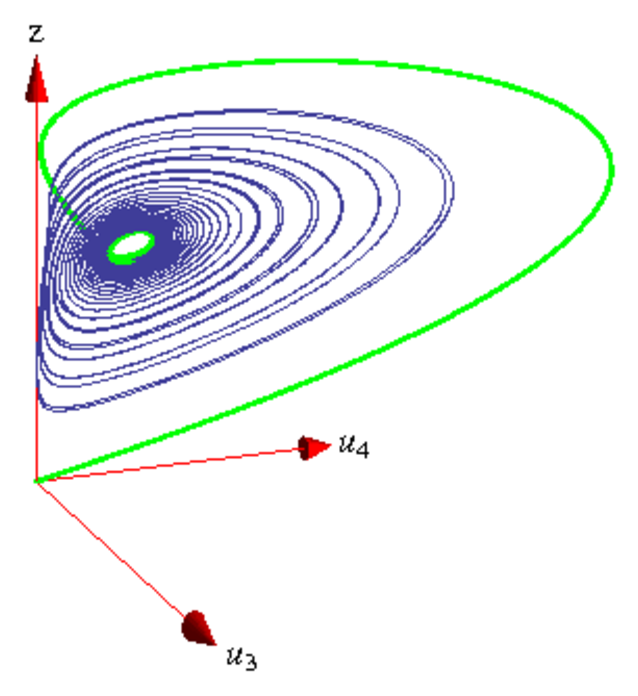
\includegraphics[width=0.35\textwidth]{../figs/CLEip1}
~~~~(\textit{b})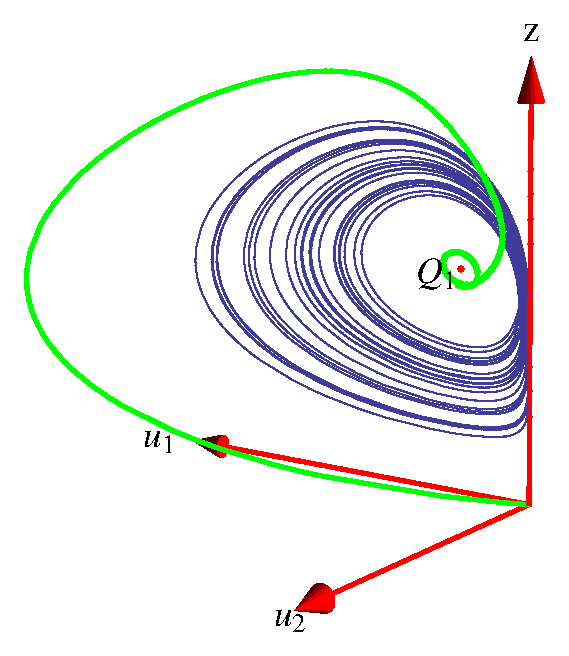
\includegraphics[width=0.36\textwidth]{../figs/CLEip2}
\end{center}
\caption[Orbit space projection of Complex Lorenz flow:
Invariant polynomials basis]{ \Statesp\ portraits of \cLe\
dynamics for $e=1/10$, $\ImrCLor=0$ in \reducedsp,
invariant polynomials basis \refeq{eq:ipLaser}.
    }
\label{fig:CLEip}
\end{figure}
%%%%%%%%%%%%%%%%%%%%%%%%%%%%%%%%%%%%%%%%%%%%%%%%%%%%%%%%%%%%%%%%


We use the chain rule
\beq
 \dot{u}_i=\frac{\partial u_i}{\partial x_j}\dot{x}_j
 \,,
\ee{ChainRul}
and express the result in invariant polynomials:
    \ES{mathematica notebook:CLEtransfJac.nb
    {\bf PC:} Changed $z$ to $u_5$; have not checked the algebra}\
    \ES{Rechecked algebra by hand, keeping $\rho_2\neq 0$. $u_3$ and $u_4$ where permuted. I will have to check
		the figures for consistency.}
\beq
\begin{split}
  \dot{u}_1 &=2\,\sigma\,(u_4-u_1)\,,\\
  \dot{u}_2 &=-2\left(\,u_2 - \rho_2\, u_3 -\,(\rho_1-u_5)\,u_4\right)\,,\\
  \dot{u}_3 &=-(\sigma\, +1)\,u_3+\rho_2\, u_1+e\, u_4\,,\\
  \dot{u}_4 &=-(\sigma\, +1)\,u_4+\,(\rho_1-u_5)\,u_1+\sigma\, u_2-e\,u_3\,,\\
  \dot{u}_5 &=u_4-b\, u_5\,.
\end{split}
\label{eq:CLEip}
\eeq
For visualization purposes, rather than \ESedit{integrating
\refeq{eq:CLEip}, we map solutions of \refeq{eq:CLe} to the
$u_i$'s}, \reffig{fig:CLEip}. In most projections the folding
mechanism is hidden from view since the dynamics is squeezed
near the $z$-axis.

Nevertheless we can now easily identify a suitable Poincar\'e
section as one that contains the $z$-axis and
the \reqv, here defined by the condition $u_1=u_4$.
We construct the first return map using as coordinate the
Euclidean length along the intersection of the unstable
manifold of \REQV{}{1} with the Poincar\'e surface of section,
measured from \REQV{}{1}, see \reffig{fig:CLEipRM}.


%%%%%%%%%%%%%%%%%%%%%%%%%%%%%%%%%%%%%%%%%%%%%%%%%%%%%%%%%%%%%%%%%%
\begin{figure}[ht]
\begin{center}
%   (\textit{a})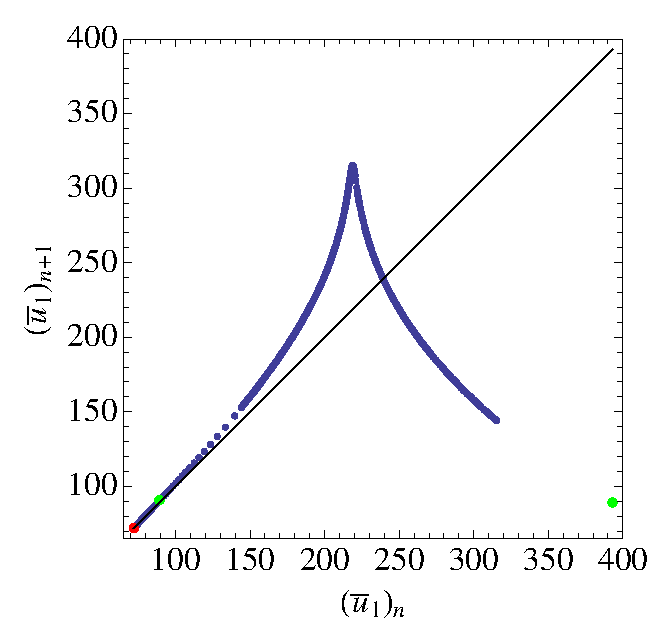
\includegraphics[width=0.35\textwidth]{../figs/CLEipRMu1}
%  ~~~~(\textit{b})
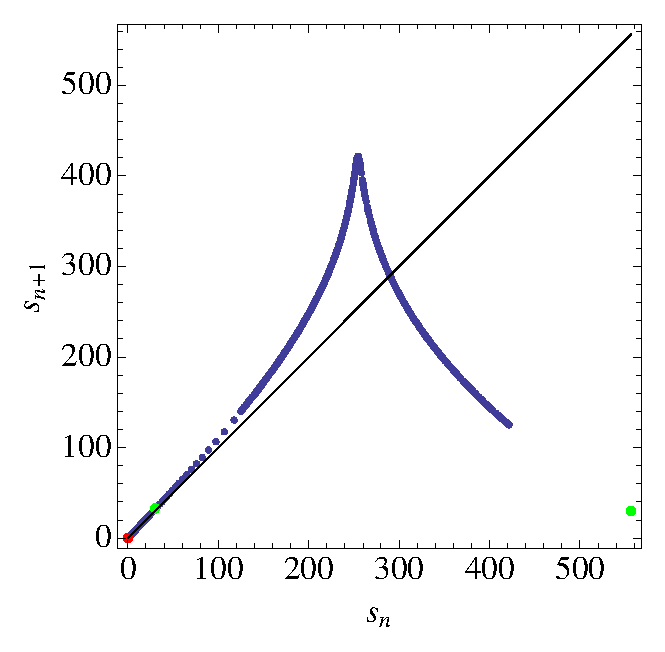
\includegraphics[width=0.35\textwidth]{../figs/CLEipRM}
\end{center}
\caption[Return map for Complex Lorenz flow, invariant polynomials]
{Return map to the \Poincare\
surface of section $u_1=u_4$ for \CLe\ with $e=1/10$, $\ImrCLor=0$,
projected on invariant polynomials \refeq{eq:ipLaser}.
% (a) The return map coordinate is $u_1$, (b)
The return map coordinate is the Euclidean
length along the \Poincare\ section of the unstable manifold of $E_1$.
    }
\label{fig:CLEipRM}
\end{figure}
%%%%%%%%%%%%%%%%%%%%%%%%%%%%%%%%%%%%%%%%%%%%%%%%%%%%%%%%%%%%%%%%


\ES{dropped, not sure it is true and it is not important anyway: 
When one takes syzygies into account in rewriting the
dynamical system, singularities are introduced. For instance
if we solve \refeq{eq:syzLaser} for $u_2$ and substitute into \refeq{eq:CLEip}
the latter reads
\beq
\begin{split}
  \dot{u}_1 &=2\,\sigma\,(u_4-u_1)\,,\\
  \dot{u}_2 &=-2\left(\,\frac{u_3^2+u_4^2}{u_1} - \rho_2\, u_3 -\,(\rho_1-u_5)\,u_4\right)\,,\\
  \dot{u}_3 &=-(\sigma\, +1)\,u_3+\rho_2\, u_1+e\, u_4\,,\\
  \dot{u}_4 &=-(\sigma\, +1)\,u_4+\,(\rho_1-u_5)\,u_1+\sigma\, \frac{u_3^2+u_4^2}{u_1}-e\,u_3\,,\\
  \dot{u}_5 &=u_4-b\, u_5\,
\end{split}
\label{eq:CLEipSyz}
\eeq
clearly singular as $u_2\rightarrow 0$. 


Moreover when
one \emph{lifts} the dynamics from the quotient space
$\Manif/G$ to the original space $\Manif$ the transformations
have singularities at the \fixedsp s of
the isotropy subgroups in $\Manif$, in the optimal case, \cf
\refref{GL-Gil07b}. Those singularities do not seem to
restrict our ability to use invariant polynomials to obtain
symmetry reduced projections of the dynamics.
}%end ES dropped text

What restricts the utility of Hilbert basis methods is that the
determination of a Hilbert basis becomes computationally
prohibitive as the dimension of the system or of the group
increases\rf{gatermannHab,ChossLaut00} and typically
computations are constrained to dimension smaller than ten. As
our goal is to quotient continuous symmetries of
high-dimensional flows, specifically those arising from
truncations of the \KS\ and Navier-Stokes flows
and thus we need an efficient framework.




